\documentclass{natureprintstyle}
%\documentclass{nature}
\bibliographystyle{naturemag}
\usepackage{epsfig,caption}
\usepackage{color}
\usepackage{bm}
\usepackage{graphicx}
\usepackage{longtable}
\usepackage{amssymb}
\usepackage{rotating}
\usepackage{latexsym}
\usepackage{hyperref}
\usepackage{float}

%\usepackage[switch]{lineno}
%\linenumbers

%%%%%%%%%%%%%%%%%%%%%%%%%%%%%%%%%%%%%%%%%%%%%%%%%%%%%%%%%%%%%%%%%%%
% comment for selecting the best figures to go on web for:
%@arxiver{jvds_sami_vsigma_ellip_LOESS_Age_paper.pdf,jvds_sami_vsigma_ellip_LOESS_Age_transform_paper_resubmit.pdf} 
%%%%%%%%%%%%%%%%%%%%%%%%%%%%%%%%%%%%%%%%%%%%%%%%%%%%%%%%%%%%%%%%%%%

%journal commands
\newcommand{\apj}{Astrophys. J.}
\newcommand{\spie}{Proc. SPIE}
\newcommand{\pasp}{Publ. Astron. Soc. Pac.}
\newcommand{\apjs}{Astrophys. J. Supp.}
\newcommand{\araa}{Annu. Rev. Astron. Astrophys.}
\newcommand{\mnras}{Mon. Not. R. Astron. Soc.}
\newcommand{\apjl}{Astrophys. J. Let.}
\newcommand{\aap}{Astron. Astrophys.}
\newcommand{\aj}{Astron. J.}
\newcommand{\nat}{Nature}
\newcommand{\na}{New Astron. Rev.}
\newcommand{\aaps}{A\&AS}
\newcommand{\procspie}{Proc. SPIE}

%%%%%%%%%%%%%%%%%%%%%%%%%%%%%%%%%%%%%%%%%%%%%%%%%%%%%%%%%%%%%%%%%%%
% my commands

\newcommand{\lcdm}{$\Lambda$CDM}
\newcommand{\hst}{{\it HST}}
\newcommand{\efr}{$R_{\mathrm{eff}}$}
\newcommand{\galfit}{{\sc Galfit}}
\newcommand{\mbh}{$\mathcal M_{\rm BH}$}
\newcommand{\lhost}{$L_{\rm host}$}
\newcommand{\jcap}{Journal of Cosmology and Astroparticle Physics}
\newcommand{\halpha}{${\it H}\alpha$}
\newcommand{\hbeta}{${\it H}\beta$}
\newcommand{\sersic}{S\'ersic}
\newcommand{\lenstronomy}{{\sc Lenstronomy}}
\newcommand{\reff}{{$R_{\mathrm{eff}}$}}
%\newcommand{\kms}{km~s$^{\rm -1}$}
\newcommand{\kms}{\ifmmode{\,\rm{km}\, \rm{s}^{-1}}\else{$\,$km$\,$s$^{-1}$}\fi}
\newcommand{\sigstar}{{$\sigma_*$}}
\newcommand{\mstar}{{$M_*$}}
\newcommand{\Mgii}{Mg$_{\rm II}$}
\newcommand{\Civ}{C$_{\rm IV}$}
%%%%%%%%%%%%%%%%%%%%%%%%%%%%%%%%%%%%%%%%%%%%%%%%%%%%%%%%%%%%%%%%%%%

\title{
%From predictions to observation: scaling relations between supermassive black holes and their host galaxies at $1< z<2$
A successful observational test of black hole and galaxy co-evolution models since $z\sim1.7$
%The first comparison between the observation and simulation of the scaling relations between supermassive black holes and their host galaxies at $1.2< z<1.7$
}
\author{Xuheng Ding$^{1}$, 
Tommaso Treu$^{1,2}$, 
John Silverman$^{1}$,
et. al
}

\begin{document}

\maketitle

\let\thefootnote\relax\footnote{
\begin{affiliations}
\item {Department of Physics and Astronomy, University of California, Los Angeles, CA, 90095-1547, USA} 
\item {School of Physics and Technology, Wuhan University, Wuhan 430072, China}
\item {Kavli Institute for the Physics and Mathematics of the Universe, The University of Tokyo, Kashiwa, Japan 277-8583 (Kavli IPMU, WPI)}
\end{affiliations}
}

\begin{abstract}
Supermassive black holes (BH) harbor at the center of galaxies with their masses correlated to the properties of the host galaxies known as scaling relations (\mbh-\lhost and \mbh-\mstar). Observational evidence indicates the correlation is evolving with cosmic time, suggesting a scenario that the BH growth predates their host. In theory, current simulations have reproduced the relations match very close to the observational sample at low redshift ($z<1$) and local. Moreover, the positive evolution of the scaling relation is predicted by different simulating projects independently. It is important to make an unbiased comparison between the observations and the simulations at higher redshift ($z>1$), where the scaling relation is predicted to have the stronger evolution. To this end, here we use a large sample of 32 X-ray-selected broad-line (type-1) AGNs at $1.2 < z < 1.7$ and compare to the predicted sample from two state-of-the-art simulating projects, MassiveBlack-II (MBII) and semi-analytic models (SAMs). We use HST to measure the luminosity of the 32 AGNs in multi-bands, hence derive the trustworthy stellar mass measurements. The \mbh\ of our sample are estimated by the published near-infrared spectroscopic observations of the broad \halpha\ and \hbeta\ emission lines. We compare the scaling relations to the simulating ones based on the same selecting function. We find that our measurements of \mbh-\lhost\ and \mbh-\mstar\ closely match to the simulations. This consistency confirms the successful progress made by the simulations, which in turn would help to understand questions such as the origin of the scaling relation, the role of AGN feedback play, and the stellar components of galaxies which directly correlate to the BH growth.
\end{abstract}

\section{Introduction}
The discovery of the correlations between the masses (\mbh) of supermassive black holes (BHs) and the properties of their host galaxies, like stellar mass (\mstar) and luminosity (\lhost), indicates that the growth of BH is linked to its host galaxy formation. The best way to understand the physical mechanism of this connection is to rely on active galactic nuclei (AGN) and trace the scaling relations to higher redshifts, witnessing how and when does it happen.

More recently, there is increasing observational evidence indicating the positive offset exist in the correlation at intermediate redshift range ($0.3<z<1$), implying that galaxies built up around the massive potential wells of mature BHs. Stimulated by the observations, theoretical efforts have been made to include the growth of \mbh\ in the framework of cosmological galaxy formation simulations, and generated the predictions of local scaling relations which match the observations well. Moreover, the simulations predict that the positive offset could be even stronger at redshift range $1<z<2$. 

A direct comparison between the observation and the simulation at high redshift range is beneficial in particular. First, it helps to directly verify the validity of the initial assumptions adopted in the simulation process, and point out the direction to improve in the simulations if needed. Second, in turn, the tested simulations could help to investigate the mechanism of the origin of the scaling relation. For example, the feedback originating in the surroundings of BHs, the major merging activities, and the growth of the \mbh\ and the stellar components as connected to the common gas supply have been invoked as the process leading to the co-evolution. Moreover, since the same selection functions are adopted when comparing the observational measurements to the predictions, the systematic bias lead by the selection effects could thus be avoided.

We study the scaling relations using 32 AGN systems from four X-ray coverage fields, including COSMOS (Civano et al. 2016), (E)- CDFS-S (Lehmer et al. 2005; Xue et al. 2011), and SXDS (Ueda et al. 2008) at redshift range $1.2<z<1.7$. We adopt the HST/WFC3 to obtain imaging data and preform the 2-D flux profile decomposition to infer the host galaxy flux value. The X-ray selected sample have low nuclear-to-host ratios, which facilitates the extraction of their host properties. 21/23 systems have HST/ACS observation, which provides the colors. Also, we combining the inference with the ground-based photometry to carry out their SED fitting, and thus derive the reliable host rest-frame R band luminosity and stellar mass. The \mbh\ of our sample are estimated using the published near-infrared spectroscopic observations of the broad \halpha\ and \hbeta\ emission lines.

We compare the obtained scaling relations to two state-of-art simulating projects, MassiveBlack-II (MBII) and semi-analytic models (SAMs). They are based on two independent simulating strategies, i.e. N-body simulation for MBII and semi-analytic model SAMs. The MassiveBlack-II (MBII) simulation is the highest resolution at the size of a comoving volume $V_{\rm box} = (100~{\rm Mpc}~h^{-1})$, including a self-consistent model for star formation, black hole accretion and associated feedback. The large simulation volume enable the simulating objects evolve independently; the high enough mass and spatial resolution meets the requirements for the object details.  On the theoretical side, aimed, high-resolution N-body simulations such as MBII can study specific galaxy systems. However, understand the mechanism of the scaling relation requires an analytical description of such processes to be implemented into existing semi-analytic models. We thus compare to the simulation based on a state-of-the-art semi-analytic models (SAMs) of galaxy formation.

\section{Results}
%Showing the result directly:
We take the same selection function as the observation to select the MBII sample at redshift range  $1.2 < z < 1.7$ to compare. 
In figure \ref{fig:MBII_comp}, we present the comparison between the observation to the simulation of the \mbh-\lhost and \mbh-\mstar. 
Inspiringly, we find that the simulation matched remarkably well to the observing result. This is the first comparison of the scaling relations at such redshift range.

\begin{figure*}%[!b]
\begin{tabular}{c c}
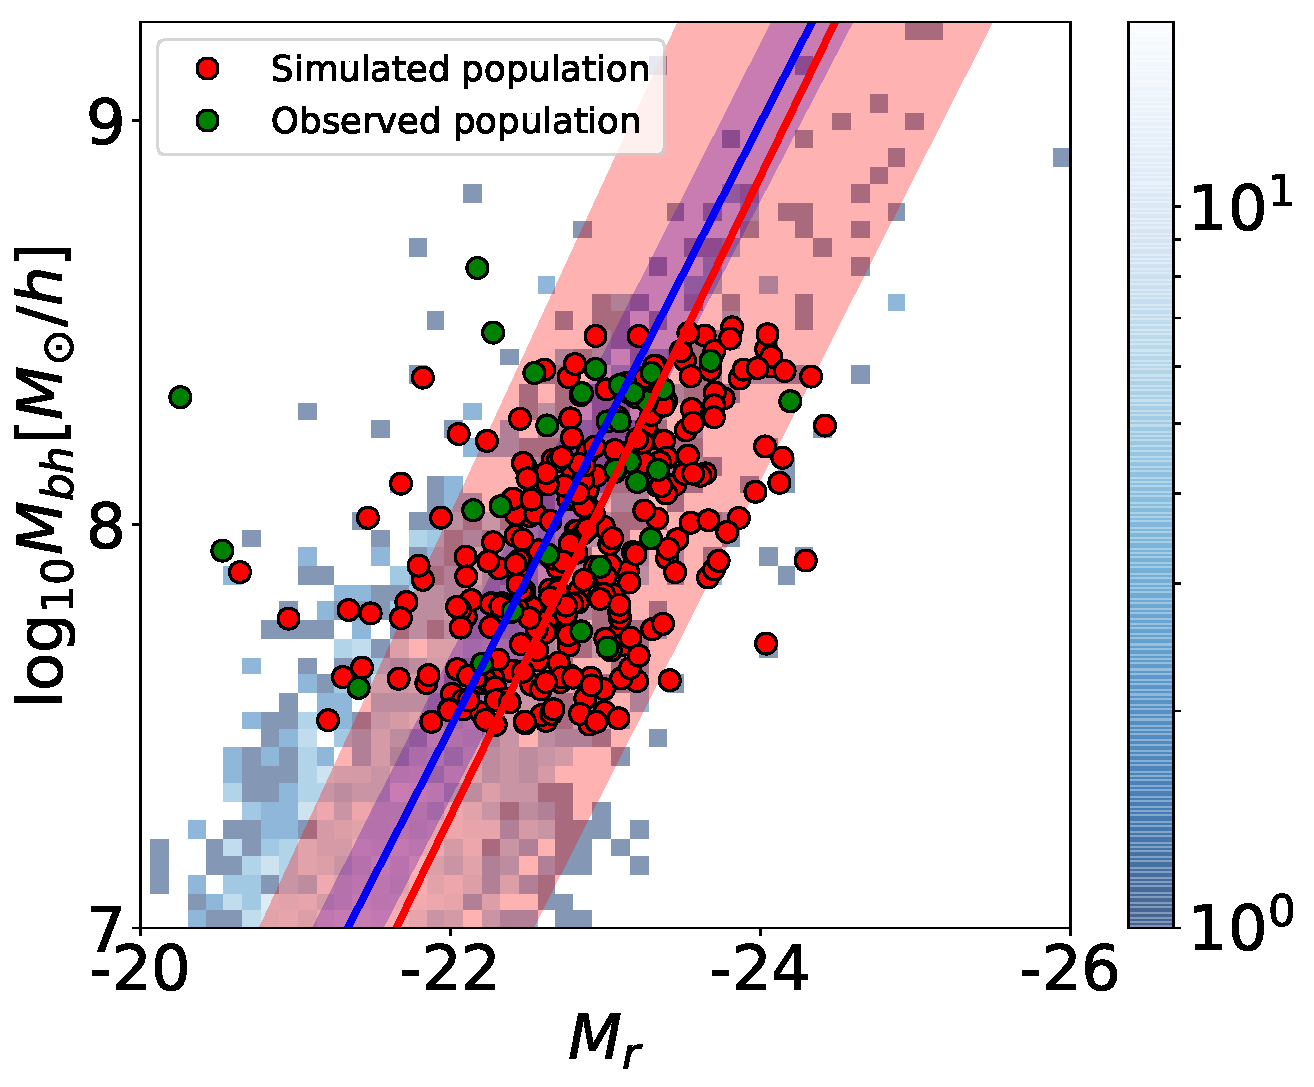
\includegraphics[width=0.5\linewidth]{MBII_ML.pdf} &
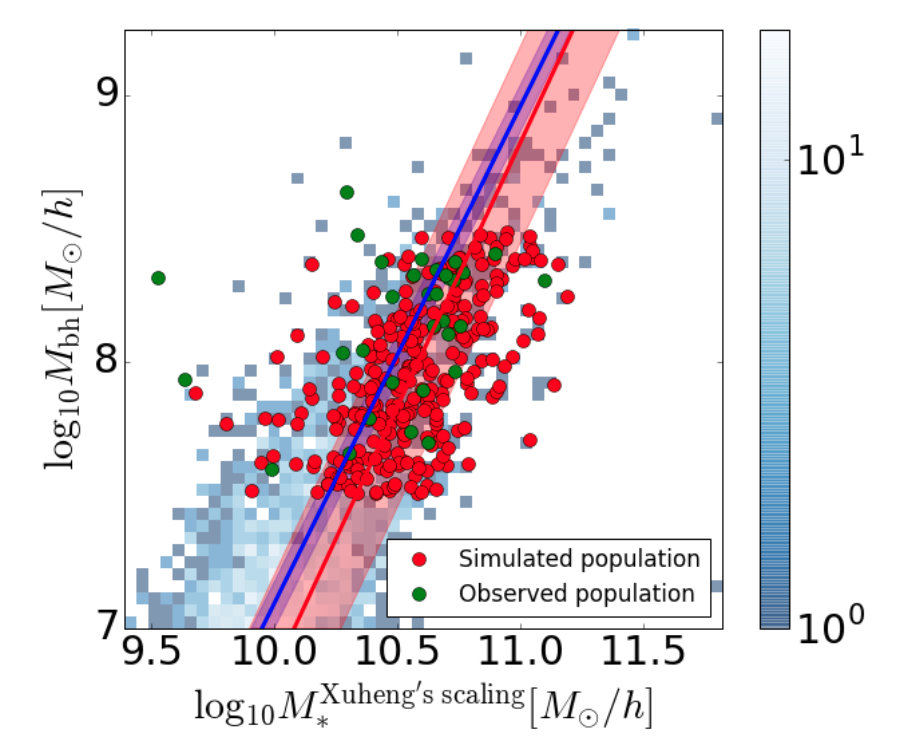
\includegraphics[width=0.5\linewidth]{MBII_MM.png} \\
\end{tabular}
\caption{
The selection function of our observation data.
Eddington ratios (LBol/LEdd) and BH masses (bottom panel) of our sample (in color) that fall well-below the knee of the BH mass function at z = 1.5 (top panel; Schulze et al. 2015). Dashed lines (vertical and horizontal) denote our selection window with the slanted line only shown to approximately illustrate the effect of a luminosity limit, inherent in the parent catalogs. For reference, we indicate the high-z luminous SDSS QSO samples (grey squares - Peng et al. 2006; grey circles - Decarli et al. 2010) with all falling above our chosen upper mass limit.
}
\label{fig:MBII_comp}
\end{figure*}

The results are presented in figure \ref{fig:SAM_comp}, demonstrating a consistency between the prediction by the model to the observation.

\begin{figure*}%[!b]
\begin{tabular}{c c}
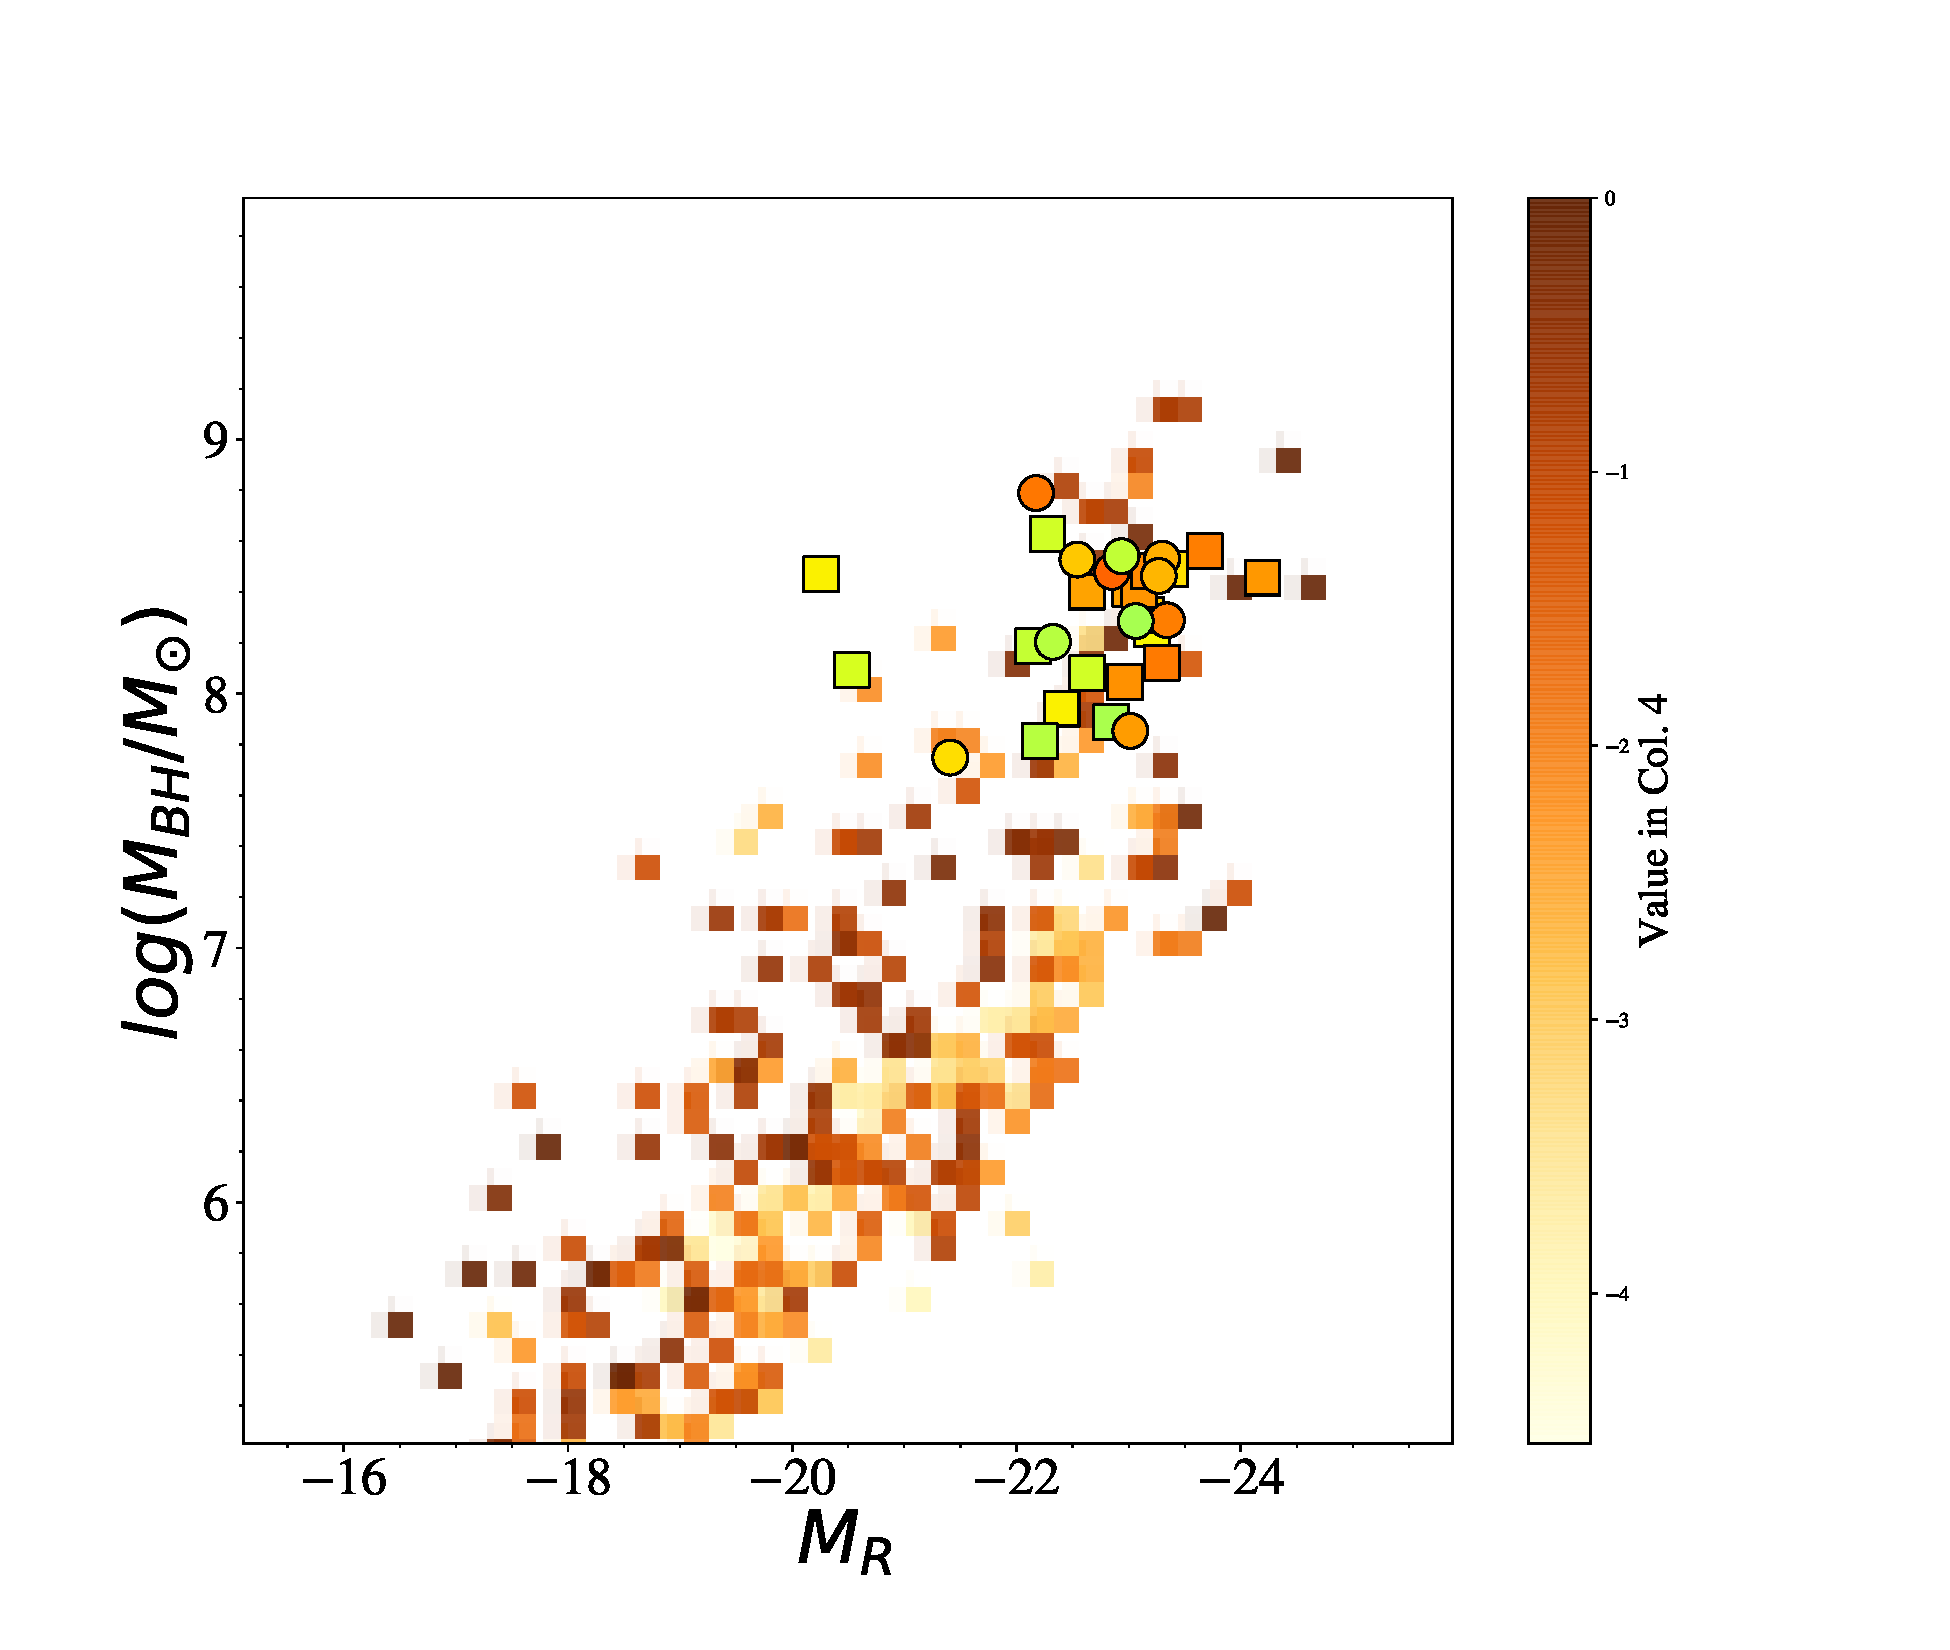
\includegraphics[width=0.5\linewidth]{SAM_ML.pdf} &
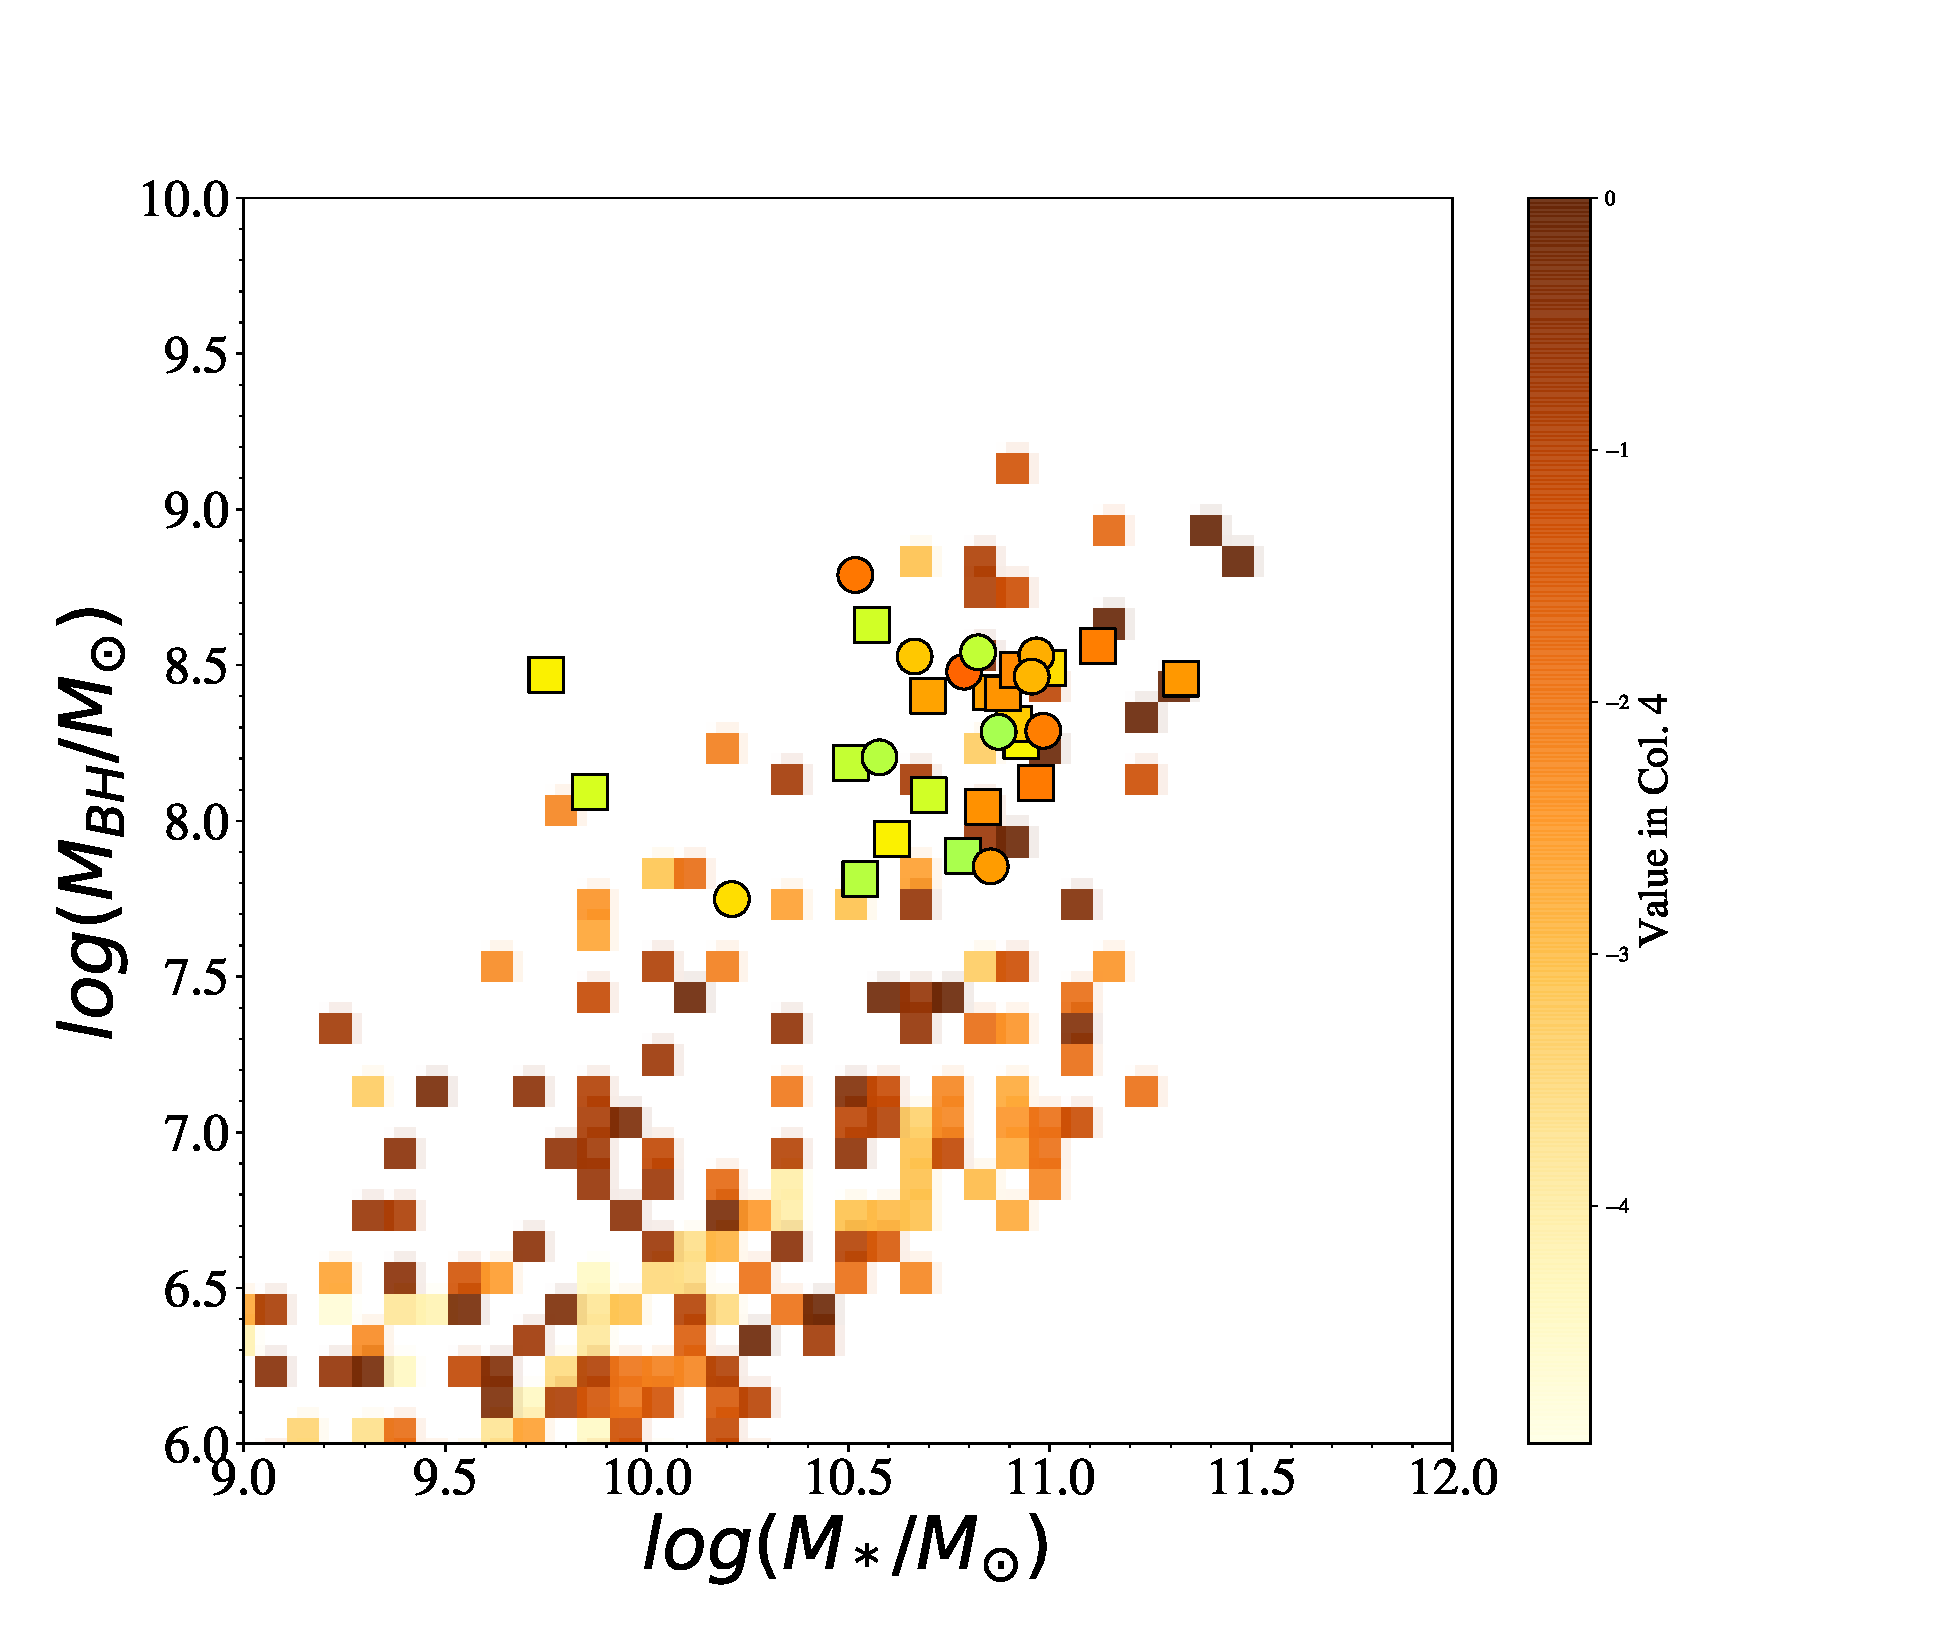
\includegraphics[width=0.5\linewidth]{SAM_MMstar.pdf} \\
\end{tabular}
\caption{
The selection function of our observation data.
Eddington ratios (LBol/LEdd) and BH masses (bottom panel) of our sample (in color) that fall well-below the knee of the BH mass function at z = 1.5 (top panel; Schulze et al. 2015). Dashed lines (vertical and horizontal) denote our selection window with the slanted line only shown to approximately illustrate the effect of a luminosity limit, inherent in the parent catalogs. For reference, we indicate the high-z luminous SDSS QSO samples (grey squares - Peng et al. 2006; grey circles - Decarli et al. 2010) with all falling above our chosen upper mass limit.
}
\label{fig:SAM_comp}
\end{figure*}

%Discuss the result.
More detailed test:
0. Compare the color of the sample?
1. KS test? 
2. More insight from the simulation?
3. Discuss the future (More sample with JWST?)

Throughout this paper, we adopt a standard concordance cosmology with $H_0= 70$ km s$^{-1}$ Mpc$^{-1}$, $\Omega{_m} = 0.30$, and $\Omega{_\Lambda} = 0.70$. Magnitudes are given in the AB system.

The ML relation that we discoverd.


\section{Discussion}


\begin{addendum}
 \item[Acknowledgements] 
X. Ding acknowledges support by China Postdoctoral Science Foundation Funded Project (No. 2017M622501).

%
\item[Correspondence] Correspondence and requests for materials should be addressed to Xuheng Ding ~(email:dxh@astro.ucla.edu).
\item[Author Contributions] xxx measure xxx, xxx extract the simulation from xx.
\end{addendum}

\clearpage
\newpage

\begin{center}
{\bf \Large \uppercase{Methods} }
\end{center}

%\textbf{Observation data.} Our 32 new AGN systems are selected from four X-ray coverage fields including COSMOS (Civano et al. 2016), (E)- CDFS-S (Lehmer et al. 2005; Xue et al. 2011), and SXDS (Ueda et al. 2008) at redshift range $1.2<z<1.7$. The X-ray selected sample have low nuclear-to-host ratios, which facilitates the extraction of the host properties. We adopt the \hst/WFC3 infrared channel to derive the high spatial resolution imaging data, to carry out the decomposition of the AGN-host using two-dimensional flux distribution. The details of the \hst\ observation and the study are presented in the companion paper. Moreover, 21/32 systems have \hst/ACS band, together with some other ground-based observations, which would provide the host information in the other bands. In the next section, we infer the reliable K-correction for the rest-frame R band luminosity and the SED to infer the stellar mass. The \mbh\ of our sample have been estimated by \halpha\ and \hbeta\ in the FMOS survey. Comparing to the \Mgii\ and \Civ, the \mbh\ by broad Balmer lines are more trustworthy. The estimated value of the \mbh\ are listed in the companion paper.
%\textcolor{blue}{Do we need to list the \mbh\ and host properties in a table in this paper?}

\textbf{Host properties inference.} We perform the 2-D AGN-host decomposition to infer the host flux. We briefly describe them here and refer the reader to the analytic paper (e.g. paper-I) for a more detailed description.

Assuming the unresolved AGN as a scaled point source and the host galaxy as a \sersic\ profile, we simultaneously fit the total 2-D flux distribution to infer the host flux ratio for the WFC3-IR data. Given that the host inference by IR band is superior to the one by UV band, we fix the \reff\ and \sersic\ index as the value inferred by WFC3-IR to infer the host ratio at ACS-UV for the 18/32 system.

We combining the HST inference to the ground-based photometry to carry out the SED fitting to infer the stellar template for each system. We adopt the best-fit SED model to derive the rest-frame R band magnitude and the stellar mass of our sample.

\textbf{Simulations and selection function.} To compare with the observation, we adopt the sample from two state-of-the-art simulating projects, i.e., MassiveBlack-II (BHII) and ab-initio semi-analytic models (SAMs).

%Introduce BHII: The high resolution. In paper?, the simulation result shows that the evolution is exists since ... Some other interesting results.
The BHII is the highest resolution at the size of a comoving volume $V_{\rm box} = (100~{\rm Mpc}~h^{-1})$, including a self-consistent model for star formation, black hole accretion and associated feedback. The large simulation volume enable the simulating objects evolve independently; the high enough mass and spatial resolution meets the requirements for the object details. A variety of predictions by the simulation have been examined by comparing to the observations, including 
the Galaxy stellar mass function, quasar bolometric luminosity function (Khandai et al. 2015). %More recently, the simulated AGN systems 
%The simulating result:
The GSMF, The AGN bol luminosity; The M-Mstar relations. The AGNs compared to the observation (Aklant two papers).

%Introduce SAMs: Similarly, the simulation of SAMs shows that, the \mbh-host relation have stronger evidence in the bulge than disk...
On the theoretical side, aimed, high-resolution N-body simulations can study specific galaxy systems, but understanding the way of AGN feeding modes requires implementing the physics of nuclear gas inflows into cosmological models of galaxy formation. In turn, this requires an analytical description of such processes to be implemented into existing semi-analytic models.

We adopt a similar selection function to allow a comparing between equivalent samples. We plot the selection function of the observation data the the simulation data, in figure.
\begin{figure}[t]
\centering
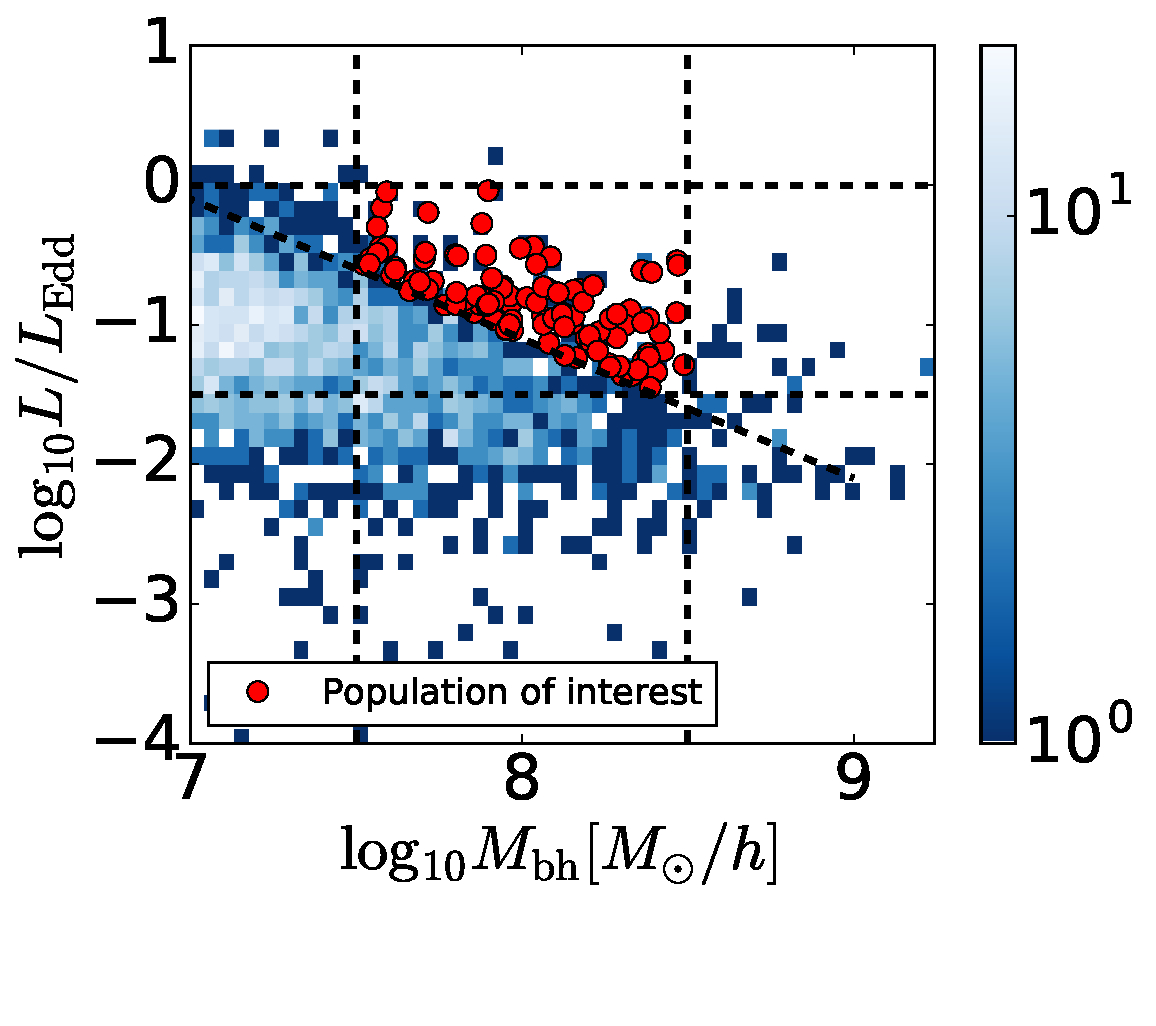
\includegraphics[width = 7cm]{MBII_selectfunc.pdf}
\caption{The sample selected from the BHII simulation.
}
\label{fig:bhII_selectfunc}
\end{figure}

\textbf{Code availability.} The data reduction package used to process the SAMI data is available at http://ascl.net/1407.006, and makes use of 2dfdr: http://www.aao.gov.au/science/software/2dfdr. To derive the stellar kinematic parameters and the lick absorption line strengths, we use the publicly available penalised pixel-fitting (pPXF) code from M. Capppellari: {http://www-astro.physics.ox.ac.uk/~mxc/software/\#ppxf}. For the adaptive LOESS smoothing, we use the code from M. Cappellari obtained from: http://www-astro.physics.ox.ac.uk/~mxc/software/\#loess

\textbf{Data availability.} All reduced data-cubes in the GAMA fields used in this Letter are available on: http://datacentral.aao.gov.au/asvo/surveys/sami/, as part of the first SAMI Galaxy Survey data release \cite{Ding2017a}. Stellar kinematic data products will become available in the second SAMI Galaxy Survey data release. 

%%%%%%%%%%%%%%%%%%%%%%%%%%%%%%%%%%%%%%%%%%%%%%%%%%%%%%%%%%%%%%%%%%%%%%%%%%%%%%%

\section*{References}
\bibliography{references} 


%%%%%%%%%%%%%%%%%%%%%%%%%%%%%%%%%%%%%%%%%%%%%%%%%%%%%%%%%%%%%%%%%%%%%%%%%%%%%%%


%%%%%%%%%%%%%%%%%%%%%%%%%%%%%%%%%%%%%%%%%%%%%%%%%%%%%%%%%%%%%%%%%%%%%%%%%%%%%%%


\clearpage
\newpage

\onecolumn

\begin{center}
{\bf \Large \uppercase{Supplementary information} }
\end{center}

\setcounter{figure}{0}
\vspace{2cm}

\begin{figure}[!h]
\begin{center}
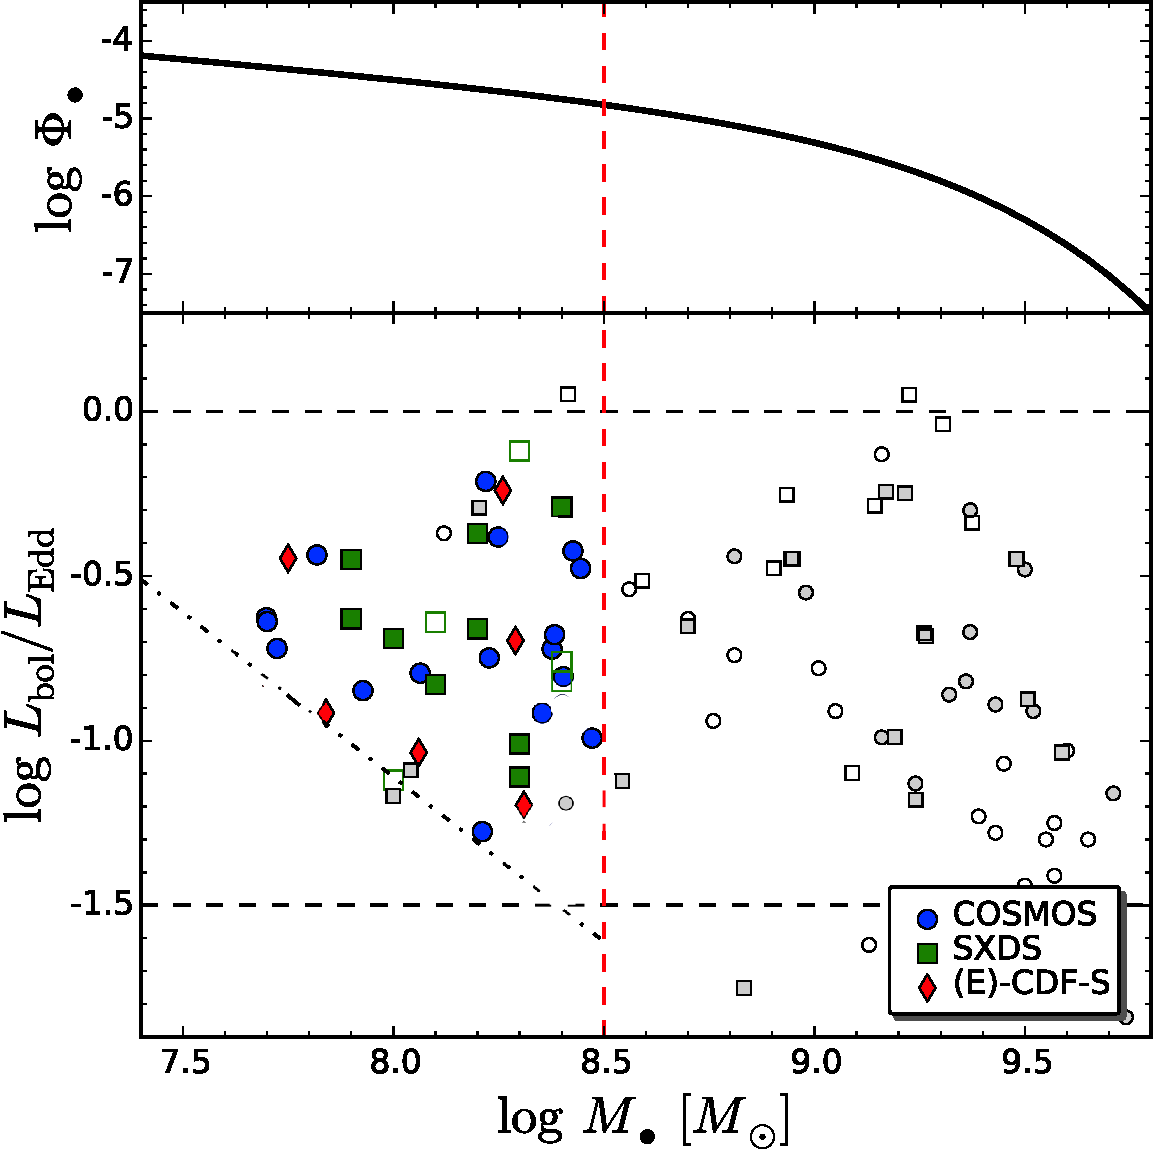
\includegraphics[width=0.8\linewidth]{hst_sample_bhmf.pdf}
\caption{
The selection function of our observation data.
Eddington ratios (LBol/LEdd) and BH masses (bottom panel) of our sample (in color) that fall well-below the knee of the BH mass function at z = 1.5 (top panel; Schulze et al. 2015). Dashed lines (vertical and horizontal) denote our selection window with the slanted line only shown to approximately illustrate the effect of a luminosity limit, inherent in the parent catalogs. For reference, we indicate the high-z luminous SDSS QSO samples (grey squares - Peng et al. 2006; grey circles - Decarli et al. 2010) with all falling above our chosen upper mass limit.
}
\label{fig:support}
\end{center}
\end{figure}


\end{document}
